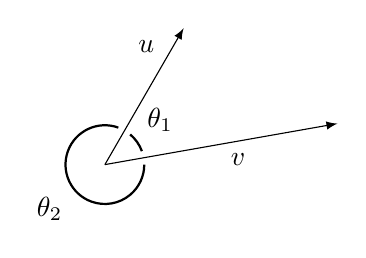
\begin{tikzpicture}[
	point/.style={circle,draw,very thin,fill,inner sep=0pt,minimum size=4pt},
	vector/.style={-latex},
]
	\draw[vector] (0,0) to node[above left,near end] {$\uvec{u}$} ++(60:2cm);
	\draw[vector] (0,0) to node[below right] {$\uvec{v}$} ++(10:3cm);
	\draw[thick] ([shift=(20:0.5cm)]0,0) arc (20:50:0.5cm) node[above right,midway] {$\theta_1$};
	\draw[thick] ([shift=(70:0.5cm)]0,0) arc (70:360:0.5cm) node[below left,midway] {$\theta_2$};
\end{tikzpicture}
